\documentclass[letterpaper,12pt]{article}
\usepackage[letterpaper, portrait, margin=0.5in]{geometry}
\usepackage{graphicx}
\usepackage{multicol}
\graphicspath{{images/}}
\newcommand\numbox{%%
    \fbox{\rule{1in}{0pt}\rule[-1ex]{0pt}{5ex}}}
\usepackage[utf8]{inputenc}
\usepackage[english]{babel}
\usepackage{multicol}
\graphicspath{{images/}{svg_images/}}
\usepackage[export]{adjustbox}

\begin{document}
\noindent Do not write your name below this line. \\
\noindent \hrule
\begin{center}
{\Large \textbf{\underline{Loops}}} \\
\end{center}
Scratch Username: \rule{4cm}{0.4pt}

\noindent \dotfill


\begin{center}
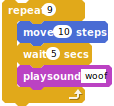
\includegraphics[scale=1]{q1_script0.png}
\end{center}
1. How many times will the blocks in the loop repeat?
\numbox \\

\noindent \dotfill
\begin{center}
\includegraphics[scale=.4]{q2_script0.png}
\end{center}

\noindent 2. \textbf{Circle} the script that makes the sprite do the same thing as the loop above: \\ \\
\includegraphics[scale=.4,valign=t]{q2_script1.png} \hspace{1.25cm}
\includegraphics[scale=.4,valign=t]{q2_script2.png} \hspace{1.25cm}
\includegraphics[scale=.4,valign=t]{q2_script3.png} \hspace{1.25cm}
\includegraphics[scale=.4,valign=t]{q2_script4.png} \hspace{1.25cm} \\

\noindent \dotfill \\

\noindent 3. \textbf{Circle \underline{ALL}} the scripts that make the sprite change costumes \textbf{exactly} 3 times. \\

\includegraphics[scale=.4,valign=t]{q3_script0.png} \hspace{1.5cm}
\includegraphics[scale=.4,valign=t]{q3_script1.png} \hspace{1.5cm}
\includegraphics[scale=.4,valign=t]{q3_script2.png} \hspace{1.5cm}
\includegraphics[scale=.4,valign=t]{q3_script3.png} \hspace{1.5cm} \\


\noindent \dotfill \\

\begin{center}
\includegraphics[scale=.4]{q4_script0.png}
\end{center}

\noindent 4a. \textbf{Circle \underline{ALL}} the blocks that run \underline{6 times} in the script above. \\ \\
\includegraphics[scale=.4]{q4_script1.png} \hspace{1cm}
\includegraphics[scale=.4]{q4_script2.png} \hspace{1cm}
\includegraphics[scale=.4]{q4_script3.png} \hspace{1cm}
\includegraphics[scale=.4]{q4_script4.png} \hspace{1cm}\\

\noindent 4b. \textbf{Circle \underline{ALL}} the blocks that run \underline{before} the repeat loop in the script above. \\ \\
\includegraphics[scale=.4]{q4_script1.png} \hspace{1cm}
\includegraphics[scale=.4]{q4_script2.png} \hspace{1cm}
\includegraphics[scale=.4]{q4_script3.png} \hspace{1cm}
\includegraphics[scale=.4]{q4_script4.png} \hspace{1cm}\\

\noindent 4c. \textbf{Circle \underline{ALL}} the blocks that run \underline{after} the repeat loop in the script above. \\ \\
\includegraphics[scale=.4]{q4_script1.png} \hspace{1cm}
\includegraphics[scale=.4]{q4_script2.png} \hspace{1cm}
\includegraphics[scale=.4]{q4_script3.png} \hspace{1cm}
\includegraphics[scale=.4]{q4_script4.png} \hspace{1cm}\\

\noindent \dotfill \\

\indent \includegraphics[scale=.45,valign=c]{cat.png} \underline{Cat's Code} \hspace{5cm}
\includegraphics[scale=.2,valign=c]{dog.png} \underline{Dog's Code} \\
\includegraphics[scale=.4,valign=t]{q5_script0.png} \hspace{1cm}
 \vline height .75cm width 2pt \hspace{1cm}
\includegraphics[scale=.4, valign=t]{q5_script1.png} \hspace{1cm}
\includegraphics[scale=.4, valign=t]{q5_script2.png} \\ \\

\noindent 5a. \textbf{Circle}: When the green flag is clicked, what will Cat do?
\renewcommand{\theenumi}{\Alph{enumi}}
\begin{enumerate}
\item Cat says "meow" 7 times \textbf{then} changes costumes 4 times.
\item Cat says "meow" and changes costumes \textbf{at the same time}. \\
\end{enumerate}

\noindent 5b. \textbf{Circle}: When the green flag is clicked, what will Dog do?
\renewcommand{\theenumi}{\Alph{enumi}}
\begin{enumerate}
\item Dog says "woof" 7 times \textbf{then} changes costumes 4 times.
\item Dog says "woof" and changes costumes \textbf{at the same time}. \\
\end{enumerate}

\newpage


\begin{center}
\includegraphics[scale=1]{q6_script0.png}
\end{center}
6. Explain what this script will make the sprite do. \\ \\
Each time the loop runs: \\ \\
\indent First \hrulefill. \\ \\
\indent Next, \hrulefill. \\ \\
\indent Last, \hrulefill. \\ \\
It does this all \rule{1cm}{0.5pt} times.

\noindent \dotfill \\
%Template for custom

\begin{center}
\includegraphics[scale=1]{q7_script0.png}
\end{center}
\noindent 7a. Why did you choose to use a loop? \\ \\
\noindent \rule{18.5cm}{0.5pt} \\ \\
\noindent \rule{18.5cm}{0.5pt} \\ \\
\noindent \rule{18.5cm}{0.5pt} \\ \\
\noindent 7b. How did you decide how many iterations (the number in the repeat loop)? \\ \\
\noindent \rule{18.5cm}{0.5pt} \\ \\
\noindent \rule{18.5cm}{0.5pt} \\ \\
\noindent \rule{18.5cm}{0.5pt} \\

\noindent \dotfill \\
Please turn the page; there is one more question!
\newpage


%Template for generic
\iffalse
\noindent 7. How do you know that you should use a loop? \\ \\
\noindent \rule{18.5cm}{0.5pt} \\ \\
\noindent \rule{18.5cm}{0.5pt} \\ \\
\noindent \rule{18.5cm}{0.5pt} \\

\noindent \dotfill \\
\fi


\begin{center}
\includegraphics[scale=.4]{ec_script0.png}
\end{center}

\noindent \textbf{Extra Challenge:} How many times will "quack" sound play? \numbox
\end{document}